%-----------------------------------------------------------------
%	INTRODUCTION
%	!TEX root = ./main.tex
%-----------------------------------------------------------------
\section{Introduction}

%-------------------------------
\subsection{The Problem}
\begin{frame}{Modelling the Kinematics I}
\begin{minipage}{.4\textwidth}
    \begin{figure}[H]
        \centering
        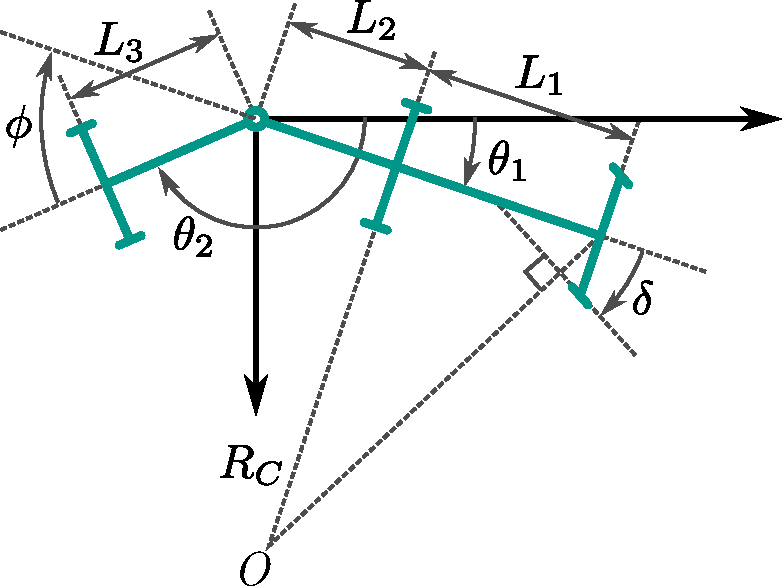
\includegraphics[width=\textwidth]{images/trailer-diagram}
        \caption{Geometric model of the car-trailer system}
        \label{fig:geom-model}
    \end{figure}
\end{minipage}%
\begin{minipage}{0.6\textwidth}
    \begin{table}[H]
        \tiny
        \centering
        \begin{tabularx}{0.95\textwidth}{c X}
            \toprule
            \toprule
            Parameters & Description \\
            \midrule
            $\theta_{1}$  & Angle of the car. \\
            $\theta_{2}$  & Angle of the trailer. \\
            $\phi$        & Angle between car and trailer. \\
            $\delta$      & Steering angle. \\
            $V$           & Speed of the car. \\
            $V_{trailer}$ & Speed of the trailer. \\
            $R_{C}$       & Distance from the centre of rotation $O$ to rear axle of the car. \\
            $L_{1}$       & Wheelbase of the car. \\
            $L_{2}$       & Overhang from the rear axle of the car to the hitch point. \\ 
            $L_{3}$       & Distance from the trailer axle to the hitch. \\ 
            \bottomrule
        \end{tabularx}
        \caption{Physical parameters of the system described by our model}
        \label{tab:parameters}
    \end{table}
\end{minipage}
\end{frame}

\begin{frame}{Modelling the Kinematics II}
\begin{minipage}{.4\textwidth}
    \begin{figure}[H]
        \centering
        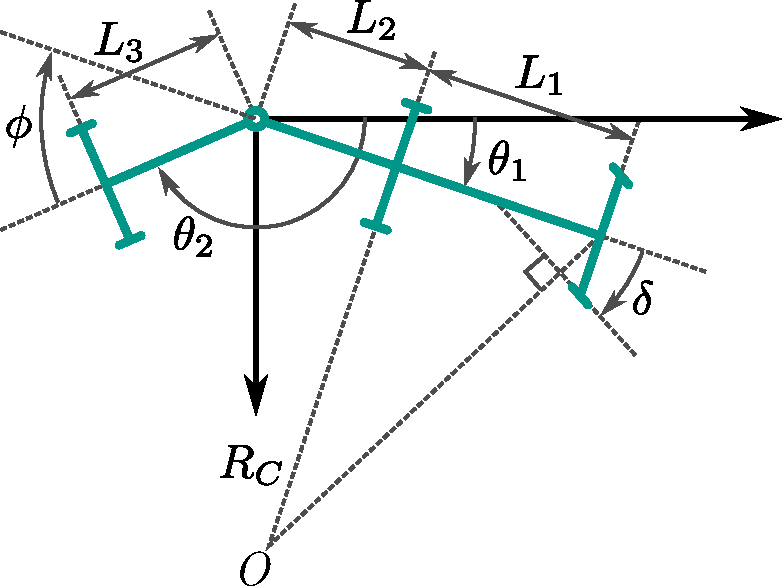
\includegraphics[width=\textwidth]{images/trailer-diagram}
        \caption{Geometric model of the car-trailer system}
        \label{fig:geom-model}
    \end{figure}
\end{minipage}%
\begin{minipage}{0.55\textwidth}
    \footnotesize
    \begin{onlyenv}<1->
    \begin{align*}
        \phi = \pi - (\theta_{2} - \theta_{1}) \qc
        \dot{\phi} = -\dot{\theta}_{2} + \dot{\theta}_{1} 
    \end{align*}
    \end{onlyenv}
    \begin{onlyenv}<+>
    \begin{align*}
        \dot{\theta}_{1} = -\frac{V}{R_{C}} \qc 
        R_C = \frac{\tan \delta}{L_1}
    \end{align*}
    \end{onlyenv}
    \begin{onlyenv}<+->
    \begin{align*}
        \dot{\theta}_{1} = -\frac{V}{L_{1}} \tan \delta 
    \end{align*}
    \end{onlyenv}
    % \begin{onlyenv}<4>
    % \begin{align*}
    %     V_{trailer} = -L_{2} \dot{\theta}_{1} \sin \phi + V \cos \phi
    % \end{align*}
    % \end{onlyenv}
    \begin{onlyenv}<+->
    \begin{align*}
        \dot{\theta}_{2} =  \frac{L_{2} \dot{\theta}_{1} \cos \phi + V \sin \phi }{L_{3}}
    \end{align*}
    \end{onlyenv}
\end{minipage}
\begin{onlyenv}<+->
\begin{align}\label{eq:dotphi-final}
    \dot{\phi} = - \frac{V}{L_{3}} \sin \phi - \frac{V}{L_{1}} \tan \delta \qty( 1 + \frac{L_{2}}{L_{3}} \cos \phi )
\end{align}
\end{onlyenv}
    
\end{frame}

%-------------------------------
\subsection{Approach}
\begin{frame}{Approaches to Solving the Problem}
\begin{itemize}
    \item Controller using pole placement
    \item Optimisation-based control
    \item Steering-based control
\end{itemize}

\end{frame}